% 0368(본책 69쪽) — ∠C=∠D=90° 인 사다리꼴 ABCD(색칠)가 반지름 5 cm 인 원 O 에 외접, AB=13 cm. 답(넓이)은 적지 않는다. 스캔 삽화를 TikZ 로 다시 그림.
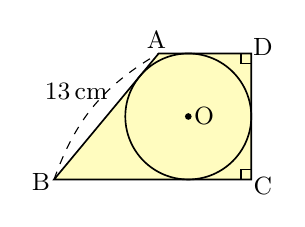
\begin{tikzpicture}[line width=0.6pt]
  \fill[yellow!25] (1.329,1.600) -- (0.000,0.000) -- (2.505,0.000) -- (2.505,1.600) -- cycle;
  \draw (1.329,1.600) -- (0.000,0.000) -- (2.505,0.000) -- (2.505,1.600) -- cycle;
  \draw (1.705,0.800) circle (0.800);
  \fill (1.705,0.800) circle (1.2pt);
  \draw[line width=0.4pt] (2.375,0.000) -- (2.375,0.130) -- (2.505,0.130);
  \draw[line width=0.4pt] (2.375,1.600) -- (2.375,1.470) -- (2.505,1.470);
  \draw[dashed, line width=0.4pt] (0.000,0.000) to[bend left=20] (1.329,1.600);
  \node[font=\small, inner sep=1.5pt] at (0.280,1.119) {$13\,\mathrm{cm}$};
  \node[font=\small, inner sep=1.5pt] at (1.300,1.767) {A};
  \node[font=\small, inner sep=1.5pt] at (-0.167,-0.030) {B};
  \node[font=\small, inner sep=1.5pt] at (2.652,-0.085) {C};
  \node[font=\small, inner sep=1.5pt] at (2.652,1.685) {D};
  \node[font=\small, inner sep=1.5pt] at (1.905,0.800) {O};
\end{tikzpicture}
